\documentclass{article}
\usepackage{iclr2027_conference,times}
\usepackage{amsmath,amssymb,booktabs,graphicx,microtype}
\usepackage{hyperref}
\usepackage{url}
\newcommand{\PrimaryDiff}{-18,220}
\newcommand{\PrimaryLow}{-19,020}
\newcommand{\PrimaryHigh}{-17,180}
\newcommand{\RunCount}{255}
\newcommand{\CPUHours}{2.54}
\newcommand{\WaitSixtyFour}{29,800}
\newcommand{\SuccessSixtyFour}{0}
\newcommand{\FitSixtyFour}{300}
\newcommand{\WaitTwoFiftySix}{11,580}
\newcommand{\SuccessTwoFiftySix}{5}
\newcommand{\FitTwoFiftySix}{100}

\title{Width and Delayed Generalization\\in Small Modular Networks}
\author{Anonymous authors}
\begin{document}
\maketitle
\begin{abstract}
Model size can affect both fitting and the discovery of algorithmic structure, making its relation to delayed generalization ambiguous. We test a strong decay-clock explanation: widening chiefly accelerates fitting, while weight decay sets a largely width-independent generalization time. We run \RunCount{} non-pilot experiments on small modular networks, with five paired seeds per grid/control cell and a separate ten-pair replication. At the reference setting, widths 64 and 256 both interpolate, but only the wider models reach sustained 95\% held-out accuracy within the horizon; their restricted mean waiting-time difference is \PrimaryDiff{} steps (95\% paired bootstrap interval [\PrimaryLow{}, \PrimaryHigh{}]). The new-seed replication gives 0/10 versus 10/10 generalization events. Matching expected initial norm preserves the contrast. Fixing hidden directions after 1,000 updates preserves training interpolation but prevents all five wide-model generalization events, whereas fixing them after 10,000 updates retains three. An explicit 61-unit ReLU circuit represents the target exactly, separating expressivity from training outcomes. These observations contradict the strong width-independent clock and support a role for continued feature learning. Width effects depend on regularization, activation, and data coverage; censored runs do not establish permanent failure, and no unique circuit mechanism is identified.
\end{abstract}

\section{Introduction}
A network can achieve almost perfect training accuracy on a small arithmetic table and only much later predict unseen entries correctly. This delayed generalization, or grokking, makes a seemingly elementary model-selection question surprisingly subtle: should a researcher use a smaller or a larger model to observe it? Increasing capacity might accelerate memorization and widen the delay, improve the discovery of reusable features and shorten it, or enable generalization that a narrower network never reaches within the budget.

These possibilities require measuring more than final accuracy or the gap between successful runs. If a narrow model memorizes but fails to generalize before a deadline, discarding it can reverse an apparent width trend. Likewise, a large model that generalizes early and a small model that cannot even fit are different failure modes for an experiment intended to exhibit grokking.

We independently construct a CPU study of modular addition with one hidden layer. Our initial explanation is deliberately strong and falsifiable: width mainly changes the fitting time, whereas regularization supplies the slower generalization clock. Fresh-seed experiments test this explanation rather than selecting only trajectories that display it. An alternative, suggested during a separate pilot, is a \emph{conditional feature-discovery account}: width changes the availability or optimization accessibility of structured solutions even after interpolation is possible, and regularization and data coverage determine which solutions are selected. This is an operational explanation, not a claim to identify a unique circuit.

Our contributions are a fully crossed width--decay comparison with explicit finite-horizon censoring; paired-seed uncertainty for waiting-time contrasts; and controls that probe whether a width effect survives initial norm matching and changes with the task or representation. All empirical figures and tables are generated from saved runs. The intended contribution is a bounded, reproducible empirical test; we do not claim a first analysis of model capacity or a complete literature survey.

\section{Related work}
\citet{power2022} introduced grokking in small algorithmically generated datasets and emphasized strong dependence on data size and regularization. Our study uses the same table-completion principle but varies hidden width in a simpler network, distinguishing fitting, delayed generalization, and right-censored runs.

\citet{nanda2023} reverse engineered Fourier-based modular-addition circuits and separated memorization, circuit formation, and cleanup. Inspired by the need for a continuous structural diagnostic, we measure output equivariance to additive shifts. This is a task-specific projection, not a reconstruction of their Transformer circuits or evidence that all our networks implement the same mechanism.

\citet{liu2023} explained grokking through a mismatch between training and test loss landscapes as a function of weight norm. \citet{varma2023} proposed competition between circuits with different norm efficiency and learning speeds. These accounts motivate our decay and norm controls. A failure of a simple decay clock would constrain a narrow interpretation of these ideas, not refute the broader theories.

\citet{kumar2024} showed that delayed feature learning can produce grokking through a transition from lazy to rich dynamics, including settings without explicit regularization. We do not measure the neural tangent kernel or infer such a transition from accuracy alone. \citet{davies2023} connected grokking and double descent through pattern learning speeds, including a capacity-dependent demonstration. Consequently, our novelty lies in the particular factorial test, censoring-aware comparison, and controls, rather than the observation that capacity can affect generalization. We use decoupled AdamW regularization as defined by \citet{adamw}.

\section{Explanations and falsifiable predictions}
\label{sec:hypotheses}
Let $T_{\mathrm{fit}}$ and $T_{\mathrm{gen}}$ denote sustained training and held-out accuracy events. The strong \emph{decay-clock explanation} says that larger width principally provides a faster route to memorization; the later transition is governed by the decay of a poorly generalizing component. A component changed only by AdamW shrinkage obeys
\begin{equation}
 v_t=(1-\eta\lambda)^t v_0,\qquad
 T_{\mathrm{shrink}}=\frac{\log(\|v_0\|/v_*)}{-\log(1-\eta\lambda)}.
 \label{eq:clock}
\end{equation}
For small $\eta\lambda$, its time scale is approximately $(\eta\lambda)^{-1}$. Equation~\ref{eq:clock} is an exact statement about pure shrinkage, not a model of the complete gradient dynamics. Applying it to grokking adds substantive assumptions about the memorizing component, its threshold, and ongoing feature learning.

We test three implications of the strong account. First, at fixed decay, increasing width should not accelerate generalization substantially more than it accelerates interpolation; otherwise width acts on the slow process as well. The primary comparison is width 64 versus 256 at $\lambda=1$. Second, when generalization occurs, $\eta\lambda T_{\mathrm{gen}}$ should approximately collapse across positive decays; a factor of two is our prechosen descriptive tolerance. Third, if width acts largely through its growing initial norm, matching that norm should substantially remove the width effect. These predictions are operational tests of the strong account; failure of one suffices to reject it in this setting.

The conditional feature-discovery account instead predicts (i) different generalization outcomes at widths that both interpolate; (ii) a width--decay interaction rather than a single width curve; and (iii) persistence of a width difference after expected initial norm matching. Rising additive-symmetry energy would be consistent with this account, but is observational evidence. We treat it as an explanation supported or challenged by interventions, not a proved necessary mechanism. The pilot informed this alternative and the setting selection; all formal seeds are distinct from the pilot seed.

\section{Experimental method}
\label{sec:method}
\paragraph{Data and model.}
For prime $p$, all ordered pairs $(a,b)\in\{0,\ldots,p-1\}^2$ are generated in lexicographic order, with label $(a+b)\bmod p$. A random permutation selects $\lfloor f p^2\rfloor$ training pairs; the remainder is the exhaustive held-out set. The reference is $p=31$, $f=0.5$, with 480 training and 481 held-out pairs. We use separate one-hot encodings of the two operands and a bias-free classifier
\begin{equation}
 z(a,b)=W_2\,\phi\!\left(W_1[e_a;e_b]\right),\quad
 W_1\in\mathbb R^{w\times 2p},\quad W_2\in\mathbb R^{p\times w}.
\end{equation}
Thus the parameter count is exactly $3pw$. Reference widths $16,32,64,128,256$ range from 1,488 to 23,808 parameters. ReLU is the reference activation. Initial weights independently follow the standard linear-layer uniform distributions $W_{1,ij}\sim U[-1/\sqrt{2p},1/\sqrt{2p}]$ and $W_{2,ij}\sim U[-1/\sqrt w,1/\sqrt w]$.

\paragraph{Expressivity check.}
A constructive oracle ReLU classifier with $2p-1$ hidden units computes addition exactly (Appendix~\ref{sec:expressivity}); an eight-unit square network also suffices. Both are evaluated exhaustively by the included code. Thus at $p=31$, the reference width-64 ReLU class contains a correct solution: its failure to generalize within the horizon is not proof of inadequate expressive capacity. The constructions encode the known formula and are not learned baselines; they need not have the same norm efficiency as the solutions preferred by training.

\paragraph{Optimization and design.}
Every run performs 30,000 full-batch cross-entropy updates with AdamW: learning rate $0.003$, $\beta=(0.9,0.999)$, $\epsilon=10^{-8}$, and constant decay applied to both matrices. There is no scheduler, dropout, minibatching, checkpoint selection, or early stopping. The main grid crosses all five widths with $\lambda\in\{0,0.3,1,3\}$ and seeds $10,\ldots,14$, giving 100 runs. Dataset partitions are paired across widths and decay within each seed; independent seed streams generate partitions, initialization, and random labels. Pairing controls the sampled partition but does not make differently shaped initial matrices identical. Each process uses one CPU thread. Reference/control batches use four workers; two-worker exploratory or replication batches can overlap, with at most six training processes sharing a four-core CPU quota.

\paragraph{Events, censoring, and delay.}
We evaluate at step zero and every 100 updates. An event requires three consecutive checkpoints at or above 99\% training accuracy or 95\% held-out accuracy; its time is the first checkpoint of the qualifying triple. This yields an effective ascertainment horizon $H=29{,}800$, because events beginning after $H$ cannot be confirmed by step 30,000. A qualifying event need not imply permanent stability; a retrospective sensitivity analysis additionally requires all remaining observed checkpoints to stay above threshold. A missing event is right censored at $H$ and is never described as proof of permanent failure. We call a confirmed event delayed if $T_{\mathrm{gen}}\ge2T_{\mathrm{fit}}$ and held-out accuracy at $T_{\mathrm{fit}}$ is at most 50\%. This definition excludes trajectories that already generalize when fitting occurs; it is an operational criterion, not a universal definition of grokking. Thresholds of 90\% and 99\% are a sensitivity analysis.

\paragraph{Independent replication.}
After completing the main grid, we specified a separate replication cohort on seeds 20--29 for widths 64 and 256 at the reference setting (twenty runs). It was motivated by the limited inferential resolution of five pairs and is reported separately rather than pooled retrospectively into the primary comparison. Its paired bootstrap uses 100,000 resamples with analysis RNG seed 20261102, and both cohorts report an exact two-sided sign test.

The primary endpoint is the restricted waiting time $\tau=\min(T_{\mathrm{gen}},H)$. Since censoring is administrative and shared, its mean is directly observable without a parametric survival model. A mean of $H$ means that no qualifying event was observed; it is not an estimated event time. We compare width 256 minus width 64 within seed. Percentile 95\% bootstrap intervals enumerate all $5^5$ resamples of the five seed pairs for the original grid. Tables also report final accuracy. For event proportions, exact binomial intervals are wide: even 5/5 has a 95\% interval of approximately $[0.478,1]$, and 0/5 has $[0,0.522]$. Seed variability includes split variability, not sampling uncertainty over a fixed held-out table. Secondary comparisons are descriptive, without a multiple-testing claim.

\paragraph{Controls.}
At $\lambda=1$, widths $32,64,128,256$ and the same five seeds test: square activation; $p=47$; $f=0.7$; multiplication $(ab)\bmod31$; independent uniform random labels; and matched expected initial norm. For norm matching, multiply only $W_1$ by $\sqrt{64/w}$. Ordinarily $\mathbb E\|W_1\|_F^2=w/3$ and $\mathbb E\|W_2\|_F^2=p/3$; the intervention makes their sum $(64+p)/3$, independent of width. It also changes initial logit scale, so it does not isolate every initialization confound. Width 64 is unchanged and reuses its reference runs. These controls add 115 distinct runs. The modulus-47 maximum has 36,096 parameters, still far below the budget. Random-label experiments preserve the input distribution and training size, while removing a reusable arithmetic target.

\paragraph{Exploratory feature-direction intervention.}
After observing the primary width divergence, we added twenty explicitly exploratory runs: widths 64/256, seeds 10--14, with hidden-row directions fixed after 1,000 or 10,000 steps. Training up to the intervention is identical to the reference. Subsequently each AdamW step is followed by
\[
 W_{1,i}\leftarrow \max\!\left(0,\frac{\langle W_{1,i},u_i\rangle}{\|u_i\|^2}\right)u_i,
\]
where $u_i$ is row $i$ at the intervention. Hidden directions cannot rotate; active units retain their ReLU activation regions, while magnitudes can shrink to zero and disable a unit. Readout weights and weight decay still change. This tests whether continued directional feature learning matters, while allowing magnitude cleanup; it is a constrained-optimization intervention, not a proof of a unique mechanism. It was not part of the original frozen experimental plan.

\paragraph{Structural diagnostic.}
For class-centered logits $F(a,b,c)=z_c(a,b)-p^{-1}\sum_jz_j(a,b)$, define
\begin{equation}
 \begin{aligned}
 g(r)&=p^{-2}\!\sum_{a,b}F\big(a,b,(a+b+r)\bmod p\big),\\
 (PF)(a,b,c)&=g((c-a-b)\bmod p),\qquad
 S=\frac{\|PF\|_F^2}{\|F\|_F^2}.
 \end{aligned}
 \label{eq:structure}
\end{equation}
$P$ is the orthogonal projection onto logits depending only on the additive residual; $S$ measures their energy share. It uses the complete input table for diagnosis, and the known addition symmetry, never for training or model selection. High $S$ alone does not imply correct predictions: $g$ can peak at a wrong residual. Nor does it establish a particular Fourier circuit. For non-addition controls this is still an addition diagnostic, not a universal algorithmic progress measure.

\section{Results}
\label{sec:results}
\subsection{The width--decay map}
\begin{figure}[t]
\centering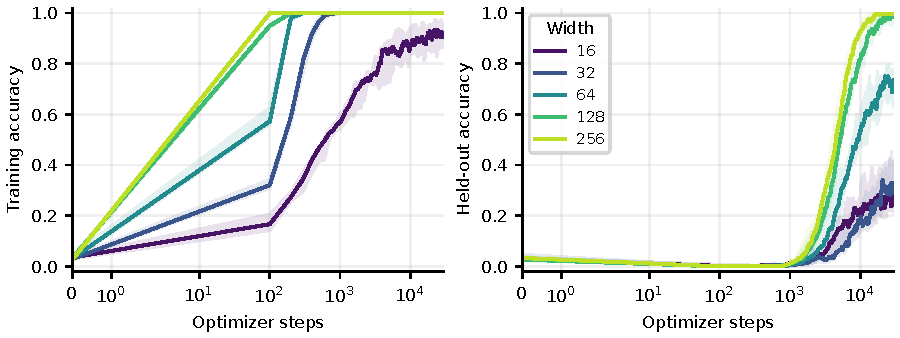
\includegraphics[width=\linewidth]{figures/curves.pdf}
\caption{Reference addition ($p=31$, $f=0.5$, $\lambda=1$). Median learning curves over all five formal seeds; shading shows the full seed range. Both training and held-out trajectories are retained through the complete training horizon.}
\label{fig:curves}
\end{figure}
\begin{table}[t]
\caption{Complete main grid. Fit, Gen., and Delayed count qualifying runs out of five; restricted waiting times include right-censored runs at $H=29{,}800$. Intervals are seed bootstrap intervals. Final held-out accuracy is measured at step 30,000.}
\label{tab:main}\centering\small
\begin{tabular}{rr rrr r r}
\toprule
$\lambda$ & Width & Fit & Gen. & Delayed & Restricted wait [95\% CI] & Final acc. \\
\midrule
0 & 16 & 5/5 & 0/5 & 0/5 & 29,800 [29,800, 29,800] & 0.012 \\
0 & 32 & 5/5 & 0/5 & 0/5 & 29,800 [29,800, 29,800] & 0.004 \\
0 & 64 & 5/5 & 0/5 & 0/5 & 29,800 [29,800, 29,800] & 0.000 \\
0 & 128 & 5/5 & 0/5 & 0/5 & 29,800 [29,800, 29,800] & 0.001 \\
0 & 256 & 5/5 & 0/5 & 0/5 & 29,800 [29,800, 29,800] & 0.004 \\
\midrule
0.3 & 16 & 4/5 & 0/5 & 0/5 & 29,800 [29,800, 29,800] & 0.023 \\
0.3 & 32 & 5/5 & 0/5 & 0/5 & 29,800 [29,800, 29,800] & 0.114 \\
0.3 & 64 & 5/5 & 0/5 & 0/5 & 29,800 [29,800, 29,800] & 0.612 \\
0.3 & 128 & 5/5 & 2/5 & 2/5 & 28,620 [26,300, 29,800] & 0.945 \\
0.3 & 256 & 5/5 & 5/5 & 5/5 & 20,360 [19,980, 20,800] & 0.994 \\
\midrule
1 & 16 & 0/5 & 0/5 & 0/5 & 29,800 [29,800, 29,800] & 0.286 \\
1 & 32 & 5/5 & 0/5 & 0/5 & 29,800 [29,800, 29,800] & 0.331 \\
1 & 64 & 5/5 & 0/5 & 0/5 & 29,800 [29,800, 29,800] & 0.716 \\
1 & 128 & 5/5 & 5/5 & 5/5 & 17,240 [15,400, 19,040] & 0.983 \\
1 & 256 & 5/5 & 5/5 & 5/5 & 11,580 [10,780, 12,620] & 0.996 \\
\midrule
3 & 16 & 0/5 & 0/5 & 0/5 & 29,800 [29,800, 29,800] & 0.034 \\
3 & 32 & 0/5 & 0/5 & 0/5 & 29,800 [29,800, 29,800] & 0.044 \\
3 & 64 & 5/5 & 0/5 & 0/5 & 29,800 [29,800, 29,800] & 0.152 \\
3 & 128 & 5/5 & 0/5 & 0/5 & 29,800 [29,800, 29,800] & 0.565 \\
3 & 256 & 5/5 & 5/5 & 5/5 & 15,520 [13,240, 16,980] & 0.951 \\
\bottomrule
\end{tabular}
\end{table}
Figure~\ref{fig:curves} and Table~\ref{tab:main} distinguish fitting from generalization. At decay 1, sustained training interpolation occurs in 0/5 runs at width 16, 5/5 runs at width 32, 5/5 runs at width 64, 5/5 runs at width 128, 5/5 runs at width 256. The corresponding generalization counts are 0/5, 0/5, 0/5, 5/5, 5/5. These observations demonstrate why a single grokking count would conflate insufficient fitting, delayed success, and unresolved generalization.

For the primary paired comparison, widths 64 and 256 have mean restricted generalization waiting times of 29,800 and 11,580 updates, respectively. The width-256 minus width-64 difference is -18,220 [-19,020, -17,180] updates (95\% paired seed bootstrap interval). Restricted training-event waiting times are 300 and 100; their paired difference is -200 [-200, -200] updates. The individual paired outcomes are in the appendix.

Widening therefore changes the slow generalization process much more than the early fitting process at the measured horizon. This contradicts the strong width-independent decay-clock explanation. The narrow model's censored time is a lower bound, so the evidence concerns finite-horizon outcomes and restricted waiting times rather than an estimated eventual event time. It does not establish permanent failure at width 64.

The original five-pair exact two-sided sign test gives $p=0.0625$. Its coarse resolution is a reason not to interpret the bootstrap interval as decisive population-level significance. An independently planned ten-pair replication on seeds 20--29 gives a restricted waiting-time difference of -18,730 [-19,190, -18,260] updates, with 0/10 versus 10/10 events and exact sign-test $p=0.0020$. The replication was designed after seeing the main-grid result and is reported as a separate cohort.

Across the full no-decay arm, 0 of 25 runs reach the generalization criterion. At positive decay, event counts depend on width and decay jointly (Figure~
ef{fig:grid}). In particular, decay 3 gives 0/5 at width 16, 0/5 at width 32, 0/5 at width 64, 0/5 at width 128, 5/5 at width 256. This comparison concerns the same step budget and fixed AdamW learning rate; it does not assert that zero decay precludes grokking under other parameterizations or longer training.

The width-256 decay-clock check reports $\eta\lambda T_{\mathrm{gen}}$, not a rescaled censored time: $\lambda=0.3$: 5/5 events, observed scaled times 17.91--18.99; $\lambda=1$: 5/5 events, observed scaled times 30.90--40.50; $\lambda=3$: 5/5 events, observed scaled times 100.80--157.50.

The ratio of largest to smallest mean scaled event time is 7.62, exceeding the prechosen factor-two descriptive tolerance. This is a diagnostic of approximate collapse, not a population equivalence test.

Among the fully observed reference widths 128 and 256, mean absolute post-fit delays are 17,040 and 11,480 steps, while mean ratios $T_{\mathrm{gen}}/T_{\mathrm{fit}}$ are 86.2 and 115.8. Thus these operational metrics have different width trends. The ratio is especially sensitive to the 100-step evaluation grid and quantization of the short fitting time; it is not evidence of an underlying continuous-time ratio law.

A three-checkpoint event need not remain above threshold. For decay 3 and width 256, 2/5 runs satisfy the additional criterion of staying above 95\% at every remaining observed checkpoint, whereas the original event count is 5/5. At decay 1, the corresponding durable-event count at width 256 is 5/5. These retrospective sensitivity results do not change the prespecified primary endpoint.


\begin{figure}[t]
\centering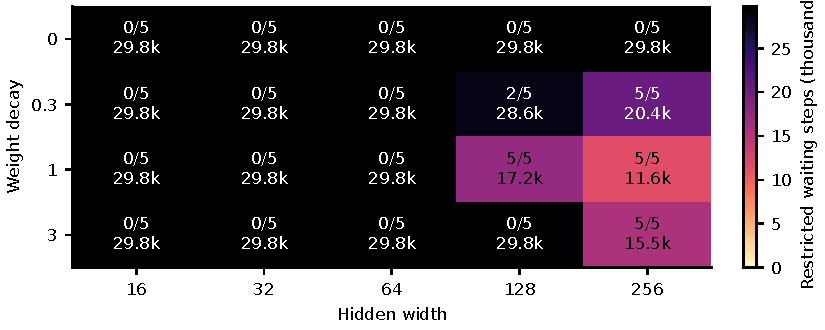
\includegraphics[width=.94\linewidth]{figures/grid.pdf}
\caption{Each cell shows the number reaching sustained 95\% held-out accuracy and mean restricted waiting time. A value of 29.8k denotes administrative censoring, not an extrapolated generalization time.}
\label{fig:grid}
\end{figure}

\subsection{Controls and scope}
\begin{table}[t]
\caption{Controls at decay 1, five seeds each. Restricted waiting times include censored runs. Mean final held-out accuracy has a 95\% seed bootstrap interval. Widths 32 and 128 are also available in the full per-run results.}
\label{tab:secondary}\centering\small
\begin{tabular}{lrrr r}
\toprule
Setting & Width & Gen. & Restricted wait & Final acc. [95\% CI] \\
\midrule
Reference ReLU & 64 & 0/5 & 29,800 & 0.716 [0.685, 0.750] \\
Reference ReLU & 256 & 5/5 & 11,580 & 0.996 [0.993, 0.999] \\
Matched initial norm & 64 & 0/5 & 29,800 & 0.716 [0.685, 0.750] \\
Matched initial norm & 256 & 5/5 & 11,020 & 0.997 [0.995, 0.999] \\
Square activation & 64 & 5/5 & 11,560 & 0.986 [0.981, 0.992] \\
Square activation & 256 & 5/5 & 12,320 & 0.984 [0.976, 0.993] \\
Addition mod 47 & 64 & 0/5 & 29,800 & 0.866 [0.841, 0.894] \\
Addition mod 47 & 256 & 5/5 & 3,840 & 1.000 [1.000, 1.000] \\
70\% training pairs & 64 & 5/5 & 17,880 & 0.952 [0.945, 0.958] \\
70\% training pairs & 256 & 5/5 & 1,660 & 1.000 [1.000, 1.000] \\
Multiplication mod 31 & 64 & 0/5 & 29,800 & 0.842 [0.830, 0.858] \\
Multiplication mod 31 & 256 & 5/5 & 11,700 & 0.994 [0.987, 0.999] \\
Random labels & 64 & 0/5 & 29,800 & 0.033 [0.029, 0.037] \\
Random labels & 256 & 0/5 & 29,800 & 0.035 [0.028, 0.042] \\
Directions fixed after 1k & 64 & 0/5 & 29,800 & 0.007 [0.004, 0.010] \\
Directions fixed after 1k & 256 & 0/5 & 29,800 & 0.022 [0.020, 0.025] \\
Directions fixed after 10k & 64 & 0/5 & 29,800 & 0.523 [0.504, 0.544] \\
Directions fixed after 10k & 256 & 3/5 & 23,060 & 0.960 [0.948, 0.973] \\
\bottomrule
\end{tabular}
\end{table}
Expected initial norm matching gives 0/5 versus 5/5 generalization events at widths 64 and 256, respectively; mean final accuracies are 0.716 and 0.997.

Replacing ReLU with a square activation gives 5/5 versus 5/5 generalization events at widths 64 and 256, respectively; mean final accuracies are 0.986 and 0.984.

Increasing the prime to 47 gives 0/5 versus 5/5 generalization events at widths 64 and 256, respectively; mean final accuracies are 0.866 and 1.000.

Increasing the training fraction to 70\% gives 5/5 versus 5/5 generalization events at widths 64 and 256, respectively; mean final accuracies are 0.952 and 1.000.

Changing addition to multiplication gives 0/5 versus 5/5 generalization events at widths 64 and 256, respectively; mean final accuracies are 0.842 and 0.994.

Replacing arithmetic labels with independent random labels gives 0/5 versus 0/5 generalization events at widths 64 and 256, respectively; mean final accuracies are 0.033 and 0.035.

Changing the modulus fixes the training fraction, not the number of examples: prime 47 uses 1,104 training pairs rather than 480, and changes both the output dimension and the parameter count at fixed width. Cross-modulus waiting times are therefore not an isolated measure of arithmetic difficulty.

These are scope and intervention tests, with uncertainty reported in Table~\ref{tab:secondary}. In particular, norm matching changes the norm trend while retaining the width intervention, but also changes the initial logit scale. Random labels test a distinct target distribution; failure to generalize there is expected and is not additional evidence for a specific arithmetic circuit. Multiplication includes zero operands and does not have the same additive translation symmetry as addition.

At the reference setting, mean final addition-symmetry energy is 0.337 at width 64 and 0.622 at width 256 (Figure~\ref{fig:diagnostics}). This diagnostic is consistent with a change in output structure when it accompanies better accuracy, but its definition already uses the task symmetry and it cannot independently establish why a feature formed.

The exploratory direction-freezing intervention after 1,000 steps gives 0/5 versus 0/5 generalization events at widths 64 and 256. Mean final training accuracies are 1.000 and 1.000, and final held-out accuracies are 0.007 and 0.022, respectively. The width-256 trajectories are shown in Appendix Figure~\ref{fig:freezing}.

The exploratory direction-freezing intervention after 10,000 steps gives 0/5 versus 3/5 generalization events at widths 64 and 256. Mean final training accuracies are 1.000 and 1.000, and final held-out accuracies are 0.523 and 0.960, respectively. The width-256 trajectories are shown in Appendix Figure~\ref{fig:freezing}.

A step advantage need not be an advantage at a common compute proxy. For a budget of $64\times30{,}000$ hidden-unit updates, the actually evaluated checkpoints are width 64 at 30,000 steps, width 128 at 15,000 steps, width 256 at 7,500 steps. Their mean held-out accuracies are 0.716, 0.928, 0.830, respectively. This proxy reflects the width-dependent dense-layer arithmetic at fixed data size; it excludes fixed framework and optimizer overhead and is not measured wall-clock equality. Full intervals and per-seed values are supplied in the appendix.


\begin{figure}[t]
\centering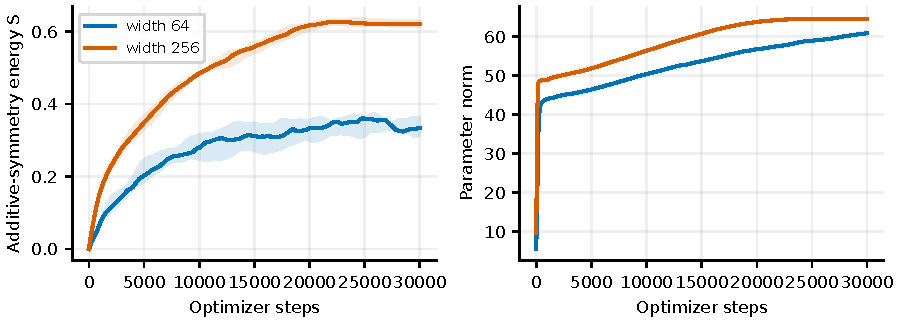
\includegraphics[width=\linewidth]{figures/diagnostics.pdf}
\caption{Addition-symmetry energy and total parameter norm at the reference decay for widths 64 and 256. Curves show medians and full seed ranges. These are diagnostic associations; no circuit-specific causal intervention is implied.}
\label{fig:diagnostics}
\end{figure}

\section{Discussion and limitations}
\label{sec:discussion}
The measured width contrast rejects the strong claim that width mainly accelerates memorization while leaving the slow process unchanged. The change occurs after both widths can fit the same training size. It is compatible with a feature-discovery bottleneck: added width changes optimization access to useful structured solutions under regularization. However, no internal circuit was isolated, and alternatives involving conditioning, redundancy, and Adam's effective updates remain possible.

Persistence of the contrast under expected initial norm matching argues against initial total norm alone as a sufficient explanation. It does not refute norm-based theories that depend on the entire optimization path or circuit efficiency.

The direction intervention supplies additional evidence: fixing hidden directions at step 1,000 preserves final training interpolation yet removes all five reference generalization events. Readout learning, individual feature magnitudes, and weight decay remain active, so their constrained continuation is insufficient from that state under these updates. Fixing directions only at step 10,000 retains 3/5 events, showing that continued direction changes are not required after that point in every observed run. The intervention still changes the optimization path, and identifies neither a unique circuit nor a general necessity theorem.

The operational distinction between occurrence and latency matters. A configuration with no confirmed event cannot be assigned a small delay; a configuration with both rapid fitting and later generalization can exhibit a large ratio even when its absolute waiting time decreases. The success map, restricted waiting time, and delayed-event counts therefore answer complementary questions. Finite-horizon success is an experimentally useful setting-selection criterion, but it is not a universal phase boundary.


This study varies hidden width in a shallow, bias-free architecture with symbolic one-hot inputs and full-batch AdamW. It does not establish a scaling law for depth, Transformers, language models, other optimizers, or natural data. Standard initialization and a fixed learning rate define the experimental intervention; changing parameterization or matching update sizes might change the relation. Matching expected total norm addresses one specific confound, but does not hold feature distributions, logits, or gradient dynamics fixed.

Finite-horizon non-generalization is a central limitation. Extending the runs could convert censored observations into delayed events and change their event-time ordering. The observed contrast in restricted waiting time remains valid for this horizon; it cannot establish that a width is incapable of eventual generalization. Five seeds permit a paired comparison but cannot tightly estimate event probabilities or rare outcomes. Bootstrap intervals from five observations are descriptive and may under-cover; a degenerate interval for all censored seeds conveys no uncertainty about performance beyond $H$. Because the whole finite operation table is evaluated, uncertainty comes from training randomness and splits, not from pretending that table entries are independent experimental replications.

The setting and alternative explanation were informed by seed-zero pilot experiments. The new-seed grid and primary contrast were fixed before those formal runs, but this is not a publicly preregistered study. The secondary controls and threshold analyses are multiple exploratory comparisons. The structural diagnostic is specific to addition and uses known task symmetry; it supports a statement about output organization, not a unique explanation of optimization. An exhaustive novelty assessment is also unavailable: literature access was deliberately restricted to the supplied starter papers to respect the independence requirement. Claims are accordingly scoped to this experiment.

\section{Conclusion}
In this finite-horizon modular study, increasing width can enable delayed generalization and markedly accelerate the slow process after training interpolation is already possible. This rejects our strong width-independent decay-clock conjecture. The width relation changes with regularization and the task controls, and initial expected norm alone is insufficient wherever the matched-norm contrast persists. The supported explanation is conditional access to structured solutions under the complete training setup, with the particular circuit mechanism and eventual outcomes beyond the horizon still unresolved.


\clearpage
\subsection*{AI use statement}
This work was performed autonomously by an AI research agent: hypothesis formation and refinement, experiment design, synthetic-data generation, mathematical definitions, implementation, analysis, literature reading, figures, and manuscript writing were AI assisted. Training and evaluation ran as real local CPU processes; measurements were not generated by a language model. Automated audits check saved checkpoints, partitions, parameter counts, numerical finiteness, event logic, and the projection identity. There has been no independent human review. Literature reading was deliberately restricted, so no exhaustive plagiarism or novelty check is claimed. This document is a research artifact using the conference format, not a claim of conference submission or acceptance.

\subsection*{Ethics statement}
The data are exhaustive synthetic arithmetic tables or locally generated random labels, with no personal information or human subjects. The principal research-integrity concerns are selective reporting, finite-horizon interpretation, and accurate attribution. We retain all pilots, interrupted-run records, raw formal measurements, and analysis code, and identify the limits of our mechanistic and novelty claims. No external publication or communication was performed.

\subsection*{Reproducibility statement}
The accompanying repository contains all configurations, training code, raw histories, final checkpoints and split indices, dependency versions, numerical audits, and figure/table scripts. Sections~\ref{sec:method} and Appendix~\ref{sec:reproduction} specify the experiments and commands. Generated \LaTeX{} tables and numerical macros are produced directly from the recorded histories. The original official ICLR 2027 style archive and author instructions are retained locally.

\bibliography{references}
\bibliographystyle{iclr2027_conference}
\clearpage
\appendix
\section{Reproduction and reporting checklist}
\label{sec:reproduction}
ICLR 2027's official template requires an AI use statement and recommends ethics and reproducibility statements; these are supplied above. The official author instructions do not prescribe a separate NeurIPS-style paper checklist. The following completed checklist records this study's reproducibility information.
\begin{enumerate}
\item \textbf{Claims and limitations: Yes.} The main text gives falsifiable predictions, distinguishes censoring from permanent failure, and restricts claims to the measured architectures and settings.
\item \textbf{Experimental design: Yes.} Model, data, split sizes, optimizer, initialization, event thresholds, evaluation frequency, and horizons are in Section~\ref{sec:method}. All runs are enumerated in \texttt{configs/main.json} and \texttt{configs/secondary.json}; the exploratory intervention is in \texttt{configs/features.json} and replication in \texttt{configs/replication.json}.
\item \textbf{Randomness and uncertainty: Yes.} Grid/control seeds are 10--14; independent replication seeds are 20--29; pilot seed is 0. Split RNG uses seed $100000+s$; random-label RNG uses $200000+s$. Intervals resample seeds; event counts and censoring are reported.
\item \textbf{Code and environment: Yes.} \texttt{requirements-lock.txt}, \texttt{environment.json}, and \texttt{README.md} give the exact observed environment and commands. No data downloads or credentials are needed to regenerate arithmetic tables.
\item \textbf{Figures and tables: Yes.} \texttt{src/analyze.py} produces all three main figures and the supplementary intervention figure, both main tables, numerical macros, sensitivity summaries, and \texttt{per\_run.csv}. \texttt{src/write\_results.py} generates empirical prose from that summary.
\item \textbf{Audits: Yes.} \texttt{src/audit.py} independently recomputes final checkpoint accuracy, verifies disjoint and exhaustive splits, matches partitions across conditions, and checks parameter counts, numerical finiteness, sustained-event logic, and projection orthogonality. It also verifies exact agreement before feature intervention and direction preservation afterward. Audit results are included.
\item \textbf{Compute: Yes.} CPU only; four-core quota, one thread per training process, up to six simultaneous training processes sharing that quota. The \RunCount{} formal runs used \CPUHours{} measured process CPU hours for training/evaluation, excluding interpreter startup, pilots, analysis, and interrupted runs. Actual wall times are retained per run.
\item \textbf{Failures and exclusions: Yes.} All completed formal runs enter analysis. Pilots select the setting and are excluded from confirmatory counts by design. An early numerical-performance amendment caused explicit interrupted runs, documented in the research log; completed superseded artifacts are retained.
\item \textbf{Data provenance and licenses: Yes.} Datasets are generated by the included arithmetic formulas, with no external data version or third-party data license. Official template files are distributed unchanged, with their original notices.
\item \textbf{Human subjects and deployment: Not applicable.} There are no human subjects, personal datasets, or deployed systems.
\item \textbf{AI disclosure: Yes.} The required statement describes the autonomous workflow and absence of human review.
\item \textbf{Literature independence: Yes within observable access.} Only direct URLs for supplied starter papers and official formatting/administrative sources were accessed. No prohibited-paper identification or search was attempted; no known accidental encounter occurred. \texttt{RESEARCH\_LOG.md} records the access scope and failed administrative URL attempts.
\end{enumerate}

\section{Additional quantitative details}
\subsection{Individual primary outcomes}

\begin{center}

\begin{tabular}{rrrrrr}

\toprule

Seed & $T_{\rm fit}^{64}$ & $T_{\rm gen}^{64}$ & $T_{\rm fit}^{256}$ & $T_{\rm gen}^{256}$ & $\tau^{256}-\tau^{64}$ \\

\midrule

10 & 300 & $>29{,}800$ & 100 & 11,300 & -18,500 \\

11 & 300 & $>29{,}800$ & 100 & 11,100 & -18,700 \\

12 & 300 & $>29{,}800$ & 100 & 10,300 & -19,500 \\

13 & 300 & $>29{,}800$ & 100 & 11,700 & -18,100 \\

14 & 300 & $>29{,}800$ & 100 & 13,500 & -16,300 \\

\bottomrule

\end{tabular}

\end{center}

\subsection{Threshold sensitivity}

All entries give sustained held-out event times in seed order 10--14; a dash means not confirmed by $H=29{,}800$.

At threshold 90\% and width 64: --, --, --, --, --.

At threshold 90\% and width 256: 9,000, 8,800, 8,300, 9,300, 9,500.

At threshold 95\% and width 64: --, --, --, --, --.

At threshold 95\% and width 256: 11,300, 11,100, 10,300, 11,700, 13,500.

At threshold 99\% and width 64: --, --, --, --, --.

At threshold 99\% and width 256: 26,700, 15,000, 13,300, 16,200, 20,700.

\subsection{Matched arithmetic budget proxy}

Width 64, checkpoint 30,000: mean held-out accuracy 0.716 [0.685, 0.750] (95\% seed bootstrap interval); individual values 0.715, 0.694, 0.775, 0.730, 0.665.

Width 128, checkpoint 15,000: mean held-out accuracy 0.928 [0.910, 0.950] (95\% seed bootstrap interval); individual values 0.933, 0.967, 0.925, 0.900, 0.917.

Width 256, checkpoint 7,500: mean held-out accuracy 0.830 [0.796, 0.862] (95\% seed bootstrap interval); individual values 0.867, 0.807, 0.871, 0.769, 0.834.

\begin{figure}[h]

\centering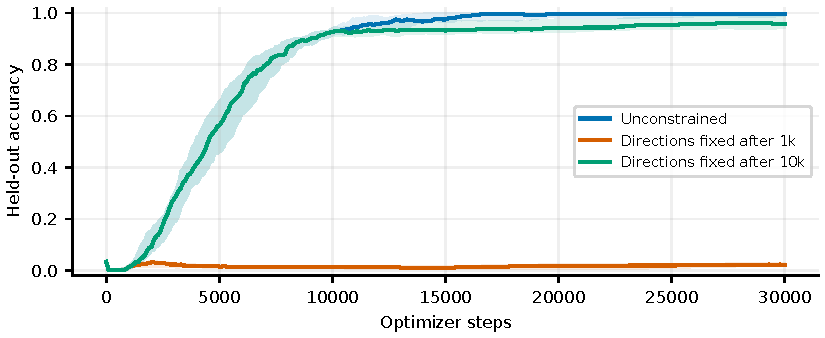
\includegraphics[width=\linewidth]{figures/feature_freezing.pdf}

\caption{Exploratory feature-direction freezing at width 256. Curves are medians with full seed ranges. The first 1,000 or 10,000 steps exactly match the unconstrained reference; subsequent optimization retains the fixed ReLU feature directions, while magnitudes and readout weights remain trainable.}

\label{fig:freezing}

\end{figure}

\subsection{Event proportions and computational cost}

Exact Clopper--Pearson intervals for every cell are in \texttt{generated/summary.json}; these intervals describe seed-level event probabilities under the complete seed-and-split procedure. Five seeds give limited resolution and no rare-event guarantee.

The 255 distinct formal runs consume 2.54 measured process CPU hours in training/evaluation. Interpreter startup, pilots, the interrupted launcher, analysis, and compilation are excluded from that total; individual measured wall times are in the raw JSON and per-run CSV.


\section{Constructive expressivity witnesses}
\label{sec:expressivity}
Let $s=a+b\in\{0,\ldots,2p-2\}$. A bias-free first-layer row with operand coefficients $a-k/2$ and $b-k/2$ produces $s-k$, because each operand is one hot. Use hidden features $h_k(s)=(s-k)_+$ for $k=-1,\ldots,2p-3$, a total of $2p-1$ units. Features with $k\ge2p-2$ are identically zero over the input domain and need not be stored. For integer $j\ge0$, set
\[
 q_j(s)=h_{j-1}(s)-2h_j(s)+h_{j+1}(s),\qquad z_c(s)=q_c(s)+q_{c+p}(s).
\]
At integer $s$ in the domain, $q_j(s)=\mathbf 1\{s=j\}$; consequently $z_c(s)=\mathbf 1\{s\bmod p=c\}$. This constructs a correct classifier within the width-64 ReLU family for $p=31$ by padding its 61 active units with zeros. It is an upper bound on required expressive width, not a lower bound or an optimization guarantee. In particular, its parameter norm can differ greatly from learned solutions.

For the square network, write $C_a=\cos(2\pi a/p)$ and $S_a=\sin(2\pi a/p)$. The eight squared linear features are $(C_a\pm C_b)^2$, $(S_a\pm S_b)^2$, $(S_a\pm C_b)^2$, and $(C_a\pm S_b)^2$. Taking pairwise differences divided by four recovers products; their linear combinations give $\cos(2\pi(a+b)/p)$ and $\sin(2\pi(a+b)/p)$. A class-dependent linear readout yields $\cos(2\pi(a+b-c)/p)$, uniquely maximized at the correct residue. The oracle uses no training data, but explicitly uses the arithmetic target.

\texttt{src/construct\_circuit.py} constructs both classifiers in float32 and verifies every ordered pair for both primes. Its measured numerical identities and accuracies are archived in \texttt{generated/expressivity.json}; it is separate from the training-run count.

\section{Pilot and numerical amendment}
The initial pilot used four 10,000-step runs (widths 64/256; ReLU/square; $p=31$, $f=0.3$, $\lambda=1$). A follow-up pilot crossed widths 32/128, fractions 0.5/0.7, activations ReLU/square, and decays 1/10 for 20,000 steps, giving sixteen further runs. Their complete raw histories and logs are retained. No pilot is counted among the formal runs. Strong decay 10 included collapsed or poorly fitting models; those results were not removed as inconvenient outcomes.

Before inspecting the main-grid outcomes, severe slowdowns associated with subnormal float32 arithmetic motivated enabling \texttt{torch.set\_flush\_denormal(True)} consistently across formal experiments. The first main launcher was stopped, its completed results archived under \texttt{results/superseded\_pre\_ftz}, and the grid restarted. Unfinished runs from that launcher are reported as interrupted rather than treated as results. Pilots retain the earlier floating-point behavior. This amendment concerns values below the normal float32 range and CPU runtime, but it is a numerical difference and is disclosed rather than silently mixed across formal cells. The final code records the setting in every formal result.
\end{document}
